\section{Транзитивное замыкание графа. Алгоритм Уоршелла. Применить алгоритм к заданному 
бинарному отношению.}

\begin{definition}
    Транзитивным замыканием бинарного отношения $R$ на
    множестве $M$ называется наименьшее по числу элементов транзитивное
    отношение на множестве $M$, включающее $R$.
\end{definition}

Если изобразить граф бинарного отношения, то транзитивность отношения
означает, что если есть ребра $(u, v), (v, w)$, то есть и ребро $(u, w)$.

На этом может быть основан алгоритм нахождения транзитивного замыкания
бинарного отношения. Для графа можно найти матрицу $T = A + A^2 + \dots + A^n$,
здесь элементы матриц складываем дизьюнктивно:
\begin{align*}
    0+0=0 \vee 0=0; \; 0+1=0 \vee 1=1; \; 1+0=1 \vee 0=1; 1+1=1 \vee 1=1. 
\end{align*}

Если элемент этой матрицы $t_{ij}=1$, то это означает, что существует маршрут от
вершины $v_i$ до $v_j$. Отсюда следует, что для транзитивности отношения эти
вершины в графе должны соединяться ребром.

Поэтому соответствующее этой матрице бинарное отношение и является его
транзитивным замыканием.

Минус этого метода в его временной сложности: временная сложность
нахождения произведения матриц размерности n равна $O(n^3)$, матрицу
смежности нужно умножать на себя n раз, поэтому временная сложность этого
алгоритма $O(n^4)$.

Есть алгоритмы, сложность которых меньше. Опишем один из таких
алгоритмов.

\newpage
\textbf{Алгоритм нахождения транзитивного замыкания Уоршелла}.
\begin{verbatim}
T := А (матрица отношения)
for k = 1 to n do
(Внешний цикл идет по промежуточным вершинам.)
    for i =1 to n do
    (Циклы по i и j перебирают всевозможные пары.)
        for j =1 to n do
            T(i; j) := max {T(i; j), T(i; k) * T(k; j)}
            (Благодаря операции max сохраняются те связи,
            которые были}
        end for
    end for
end for
\end{verbatim}

Трудоемкость такого алгоритма будет $O(n^3)$. Цикл по k нельзя
менять с другими циклами.

\begin{figure}[h]
    \centering
    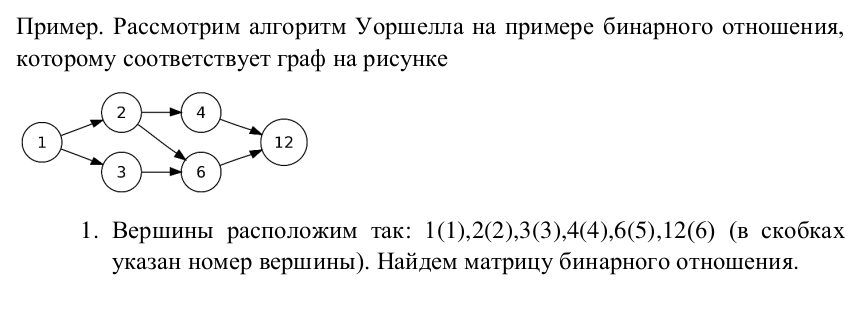
\includegraphics[scale=0.4]{19.png}
\end{figure}
\begin{figure}[h]
    \centering
    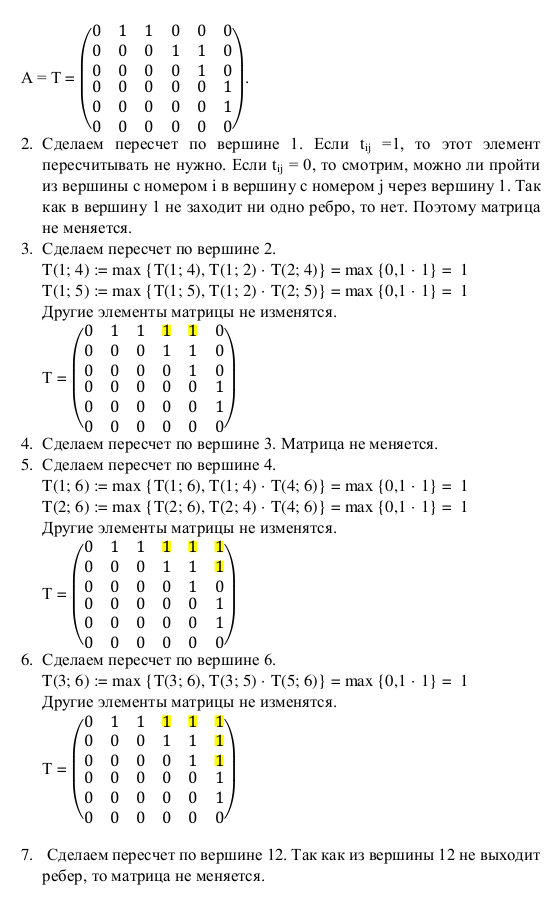
\includegraphics[scale=0.5]{19_2.png}
\end{figure}

В итоге видим, что нужно добавить 5 ребер: (1,4), (1,6), (1,12), (2,12),
(3,12).